% Pregunta heredada de E1 y alcance efectivamente ejecutado.
\section{Pregunta y alcance}
¿Dedicar parte del presupuesto a ajuste supervisado mejora el desempeño que
se obtiene con aprendizaje por refuerzo en problemas cuantitativos con unidades?
Para responderlo comparamos cuatro rutas de Qwen3-1.7B: el modelo base, el ajuste
supervisado, el refuerzo directo y el ajuste supervisado seguido de refuerzo.
El estudio mide desempeño en validación y examina si la recompensa programática
aporta señal durante el entrenamiento.

% Método: entorno, datos, rutas, cómputo y evaluación común.
\section{Implementación y protocolo}

\textbf{Entorno y datos.} Ampliamos el entorno de tres a seis familias: velocidad,
energía cinética, luminosidad, densidad, presión y tensión eléctrica. Cada tarea
presenta magnitudes, fórmula y unidad de salida. Las dificultades combinan
representaciones y conversiones distintas. Las tres variantes de cada problema
físico quedan en una sola partición. La división reúne 1.800 tareas de
entrenamiento, 360 de validación y 360 de prueba, correspondientes a 600, 120 y
120 problemas físicos, respectivamente. La prueba queda reservada para la
evaluación final.

Qwen3-8B generó cuatro soluciones candidatas por tarea de entrenamiento.
Tras verificar, deduplicar y filtrar las candidatas, retuvimos 3.362 trazas
para ajuste supervisado (SFT). Los errores numéricos identificados, complementados
con respuestas del modelo objetivo, permitieron construir 769 pares de respuestas
preferida y rechazada para optimización directa de preferencias (DPO)
\cite{dpo}. La escasez de candidatas aptas redujo la cobertura de energía y
luminosidad y dejó los volúmenes por debajo de las metas orientativas de 4.000
trazas y 2.000 pares.

\textbf{Verificación y entrenamiento.} El verificador calcula la referencia
a partir del problema. Asigna recompensa 1 si la respuesta es interpretable,
usa la unidad pedida y su error relativo es de hasta el 1\%. Las demás
respuestas reciben 0. SFT ajusta el modelo para reproducir las soluciones
retenidas. GRPO (\textit{Group Relative Policy Optimization}) compara cuatro
respuestas de un mismo problema y usa sus
recompensas relativas para ajustar el modelo \cite{deepseekmath}. La ruta
híbrida inicia GRPO desde el paso 90 de SFT, aproximadamente al 25\% del
presupuesto. DPO quedó preparado a nivel de datos.

Entrenamos adaptadores QLoRA en una RTX 3050 Laptop de 6 GiB, con un presupuesto
nominal de 1.200 s por ruta y una semilla de entrenamiento. Las tres rutas
entrenadas cambiaron 112 tensores del adaptador y recuperaron sus pesos
exactamente al recargar. El tiempo de la ruta híbrida suma SFT y GRPO. El
presupuesto se comprueba al terminar cada paso, lo que explica que los tiempos
observados excedan el nominal (tabla~\ref{tab:resultado}).

\textbf{Evaluación.} Generamos tres respuestas por tarea de validación para el
control previo al ajuste y para cada ruta al cierre, con el mismo verificador
y muestreo (temperatura 0,7, \textit{top-p} 0,9, \textit{top-k} 40 y hasta 512
tokens nuevos). Con tres intentos, \textit{pass@1} promedia la fracción de respuestas
aceptadas por tarea y \textit{pass@3} la fracción de tareas con al menos una
respuesta aceptada. Los intervalos del 95\% se obtienen por remuestreo pareado
de los 120 problemas físicos, conservando juntas sus variantes. Para medir el
desempeño entre cierres usamos 36 tareas fijas con una respuesta por tarea. En esa
muestra, el \textit{pass@1} del control fue 61,11\%.

% Resultados: mantener cifras exactas, denominadores y lectura de curvas.
\section{Resultados y señal de aprendizaje}

\begin{table}[ht]
\centering
\caption{Resultados al cierre en validación. Cada ruta produjo 1.080 respuestas
sobre 360 tareas. El costo corresponde al entrenamiento acumulado.}
\label{tab:resultado}
\begin{tabular}{lrrrr}
\toprule
Ruta & Pasos & Tiempo (s) & \textit{pass@1} (\%) & \textit{pass@3} (\%) \\
\midrule
Control & 0 & 0 & 69,44 & 84,17 \\
SFT & 377 & 1.201,81 & 76,57 & 86,11 \\
GRPO & 40 & 1.297,77 & 69,35 & 84,17 \\
SFT seguido de GRPO & $90+31$ & 1.236,85 & 73,89 & 86,94 \\
\bottomrule
\end{tabular}
\end{table}

SFT obtuvo el mayor \textit{pass@1} observado y superó al control en 7,13
puntos porcentuales (IC 95\%: 4,17 a 10,09). GRPO quedó cerca del control
($-0,09$ puntos, IC 95\%: $-1,76$ a 1,58). El híbrido superó a GRPO en 4,54
puntos (IC 95\%: 1,11 a 7,87), y quedó por debajo del SFT de presupuesto
completo. Los intervalos para las diferencias de \textit{pass@3} frente al
control incluyeron cero. El promedio de SFT reúne mejoras en densidad, presión,
velocidad y tensión, junto con caídas en energía y luminosidad. El
anexo~\ref{sec:detalle} muestra el desglose por nivel y familia.

Las curvas de recompensa (figura~\ref{fig:entrenamiento}) muestran grupos
constantes en 20 de 40 pasos de GRPO y 19 de 31 pasos del híbrido. Esos grupos
aportan ventaja relativa nula. La pérdida de SFT bajó durante el entrenamiento.
En la validación intermedia hubo oscilaciones y las dos rutas con refuerzo
carecieron de una tendencia sostenida (figura~\ref{fig:validacion}). El
punto de partida SFT del híbrido se midió en la muestra de 36 tareas. Esa
diferencia de protocolo impide cuantificar el aporte del refuerzo sobre el
ajuste supervisado inicial con la evaluación de 360 tareas.

\section{Iteraciones y auditoría}

En una prueba de desarrollo el modelo copiaba literalmente el marcador de
unidad. Indicamos la unidad solicitada en el formato de ejemplo y explicitamos
el punto decimal. En las mismas 36 tareas el \textit{pass@1} subió de 38,89\%
a 72,22\% y la proporción de respuestas interpretables pasó de 69,44\% a
100\%, usando los mismos pesos. El cambio muestra sensibilidad al formato
de la instrucción. En otro piloto, tres grupos con recompensa uniforme de
cero produjeron gradientes nulos. Las corridas posteriores registraron grupos
con recompensas mixtas y actualizaciones efectivas de los adaptadores.

La auditoría examinó datos, fórmula, conversiones, operaciones y conclusión
en una muestra estratificada de respuestas aceptadas, con hasta tres respuestas
únicas por combinación de familia, dificultad y ruta. Se revisaron además
trazas de entrenamiento SFT y respuestas de calibración. La
tabla~\ref{tab:auditoria} reúne los 287 dictámenes humanos originales:
129 casos aceptados y 158 rechazados. Entre las 53 trazas de entrenamiento
SFT, se rechazaron cinco por errores aritméticos, de conversión
o de explicación. El muestreo permite identificar tipos de defectos en los
casos inspeccionados. Las proporciones de la muestra dependen del diseño
estratificado y del número de éxitos disponibles en cada estrato.

% Cierre: interpretar la comparación sin extrapolar una semilla ni atribuir causalidad.
\section{Conclusiones}

Con este presupuesto, el ajuste supervisado logró el mayor desempeño observado
en un intento. El híbrido mejoró respecto de iniciar GRPO desde el modelo base.
Esta diferencia corresponde a una semilla y a presupuestos nominales comunes,
con distinta cantidad de pasos y un perfil energético inicial sin registrar
para el control y GRPO. La cobertura desigual de las trazas también limita la
interpretación de las diferencias por familia.

La Entrega 3 incorporará DPO, una evaluación completa del punto de partida
SFT del híbrido y un análisis de la asignación de cómputo entre fases.
Las repeticiones con otras semillas dependen del cómputo disponible.
La comparación final usará la partición reservada y un verificador común.

\clearpage
\appendix
\section{Curvas de entrenamiento y validación}
\begin{figure}[!ht]
\centering
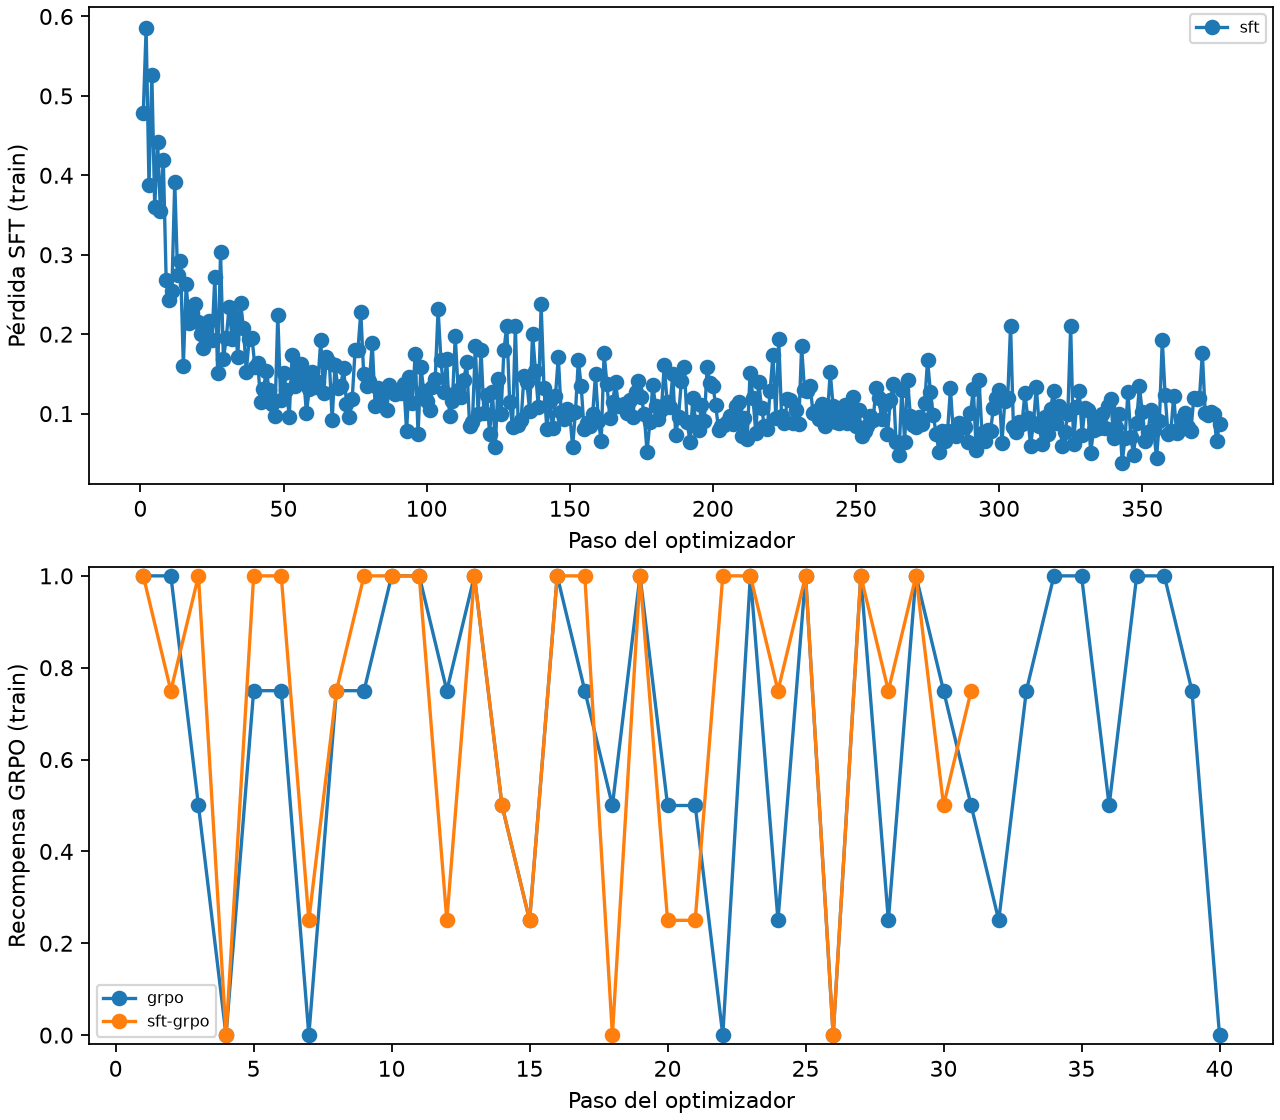
\includegraphics[width=0.82\linewidth]{figures/training-curves.png}
\caption{Arriba, pérdida de SFT por paso del optimizador. Abajo, recompensa
media del grupo de cuatro respuestas en cada paso de GRPO puro (azul) y de
la fase GRPO del híbrido (naranjo). Un promedio de 0 o 1 identifica un
grupo con recompensa constante.}
\label{fig:entrenamiento}
\end{figure}

\begin{figure}[!ht]
\centering
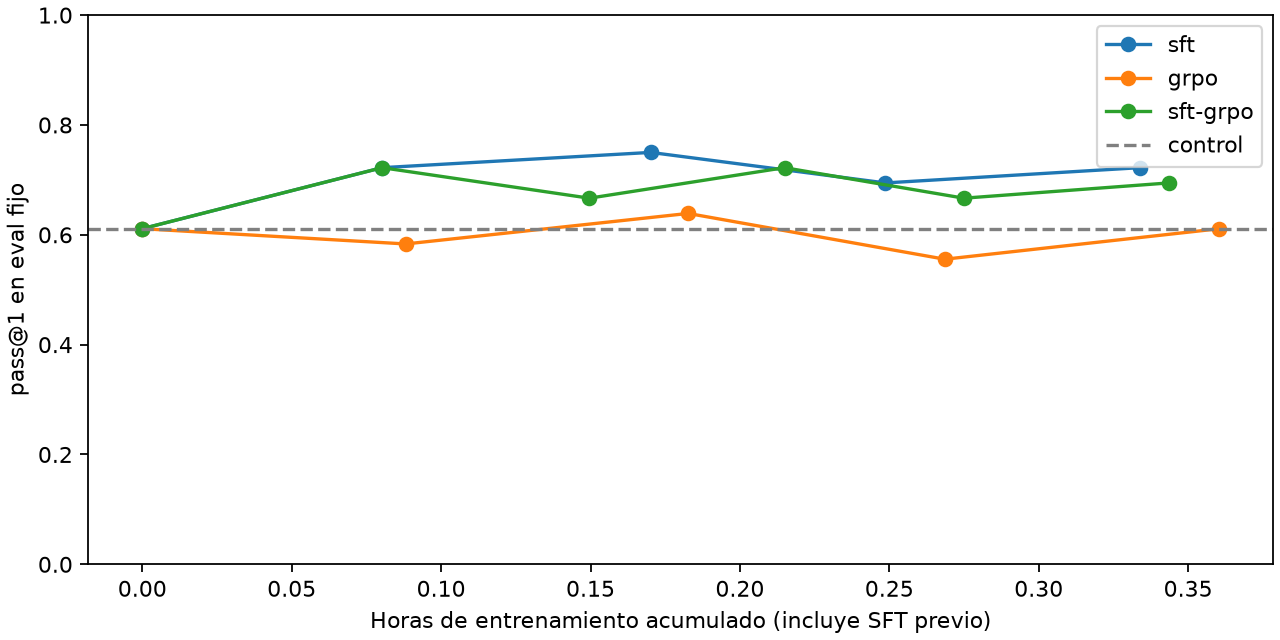
\includegraphics[width=0.82\linewidth]{figures/validation-vs-compute.png}
\caption{\textit{Pass@1} en una muestra fija de 36 tareas con un intento por
tarea, frente a horas de entrenamiento acumuladas. El tiempo híbrido
incluye 288,88 s de SFT previo. Los cierres sobre 360 tareas con tres intentos
se informan en la tabla~\ref{tab:resultado}.}
\label{fig:validacion}
\end{figure}

\clearpage
\section{Detalle de validación y auditoría}
\label{sec:detalle}
\begin{table}[ht]
\centering
\caption{Validación al cierre por dificultad. Cada nivel tiene 120 tareas y
360 respuestas por ruta. Las celdas muestran \textit{pass@1} / \textit{pass@3}
en porcentaje.}
\begin{tabular}{lrrrr}
\toprule
Dificultad & Control & SFT & GRPO & SFT seguido de GRPO \\
\midrule
Fácil & 83,89 / 96,67 & 83,89 / 91,67 & 83,61 / 95,83 & 83,33 / 93,33 \\
Media & 84,44 / 95,00 & 79,44 / 91,67 & 82,22 / 95,00 & 83,33 / 94,17 \\
Difícil & 40,00 / 60,83 & 66,39 / 75,00 & 42,22 / 61,67 & 55,00 / 73,33 \\
\bottomrule
\end{tabular}
\end{table}

\begin{table}[ht]
\centering
\caption{\textit{Pass@1} por familia al cierre (\%). Cada familia tiene
60 tareas y 180 respuestas por ruta.}
\begin{tabular}{lrrrr}
\toprule
Familia & Control & SFT & GRPO & SFT seguido de GRPO \\
\midrule
Velocidad & 86,11 & 96,67 & 88,33 & 88,33 \\
Energía & 78,33 & 60,56 & 78,33 & 60,56 \\
Luminosidad & 38,89 & 18,33 & 37,22 & 28,33 \\
Densidad & 65,56 & 98,89 & 64,44 & 90,56 \\
Presión & 76,11 & 96,67 & 77,22 & 92,22 \\
Tensión & 71,67 & 88,33 & 70,56 & 83,33 \\
\bottomrule
\end{tabular}
\end{table}

\begin{table}[ht]
\centering
\caption{Resultados de la auditoría humana por muestra.}
\label{tab:auditoria}
\begin{tabular}{lrrrr}
\toprule
Muestra & Revisados & Aceptados & Rechazados & Dudosos \\
\midrule
Control & 52 & 12 & 40 & 0 \\
SFT & 51 & 21 & 30 & 0 \\
GRPO & 53 & 25 & 28 & 0 \\
SFT seguido de GRPO & 52 & 21 & 31 & 0 \\
Calibración & 26 & 2 & 24 & 0 \\
Corpus SFT & 53 & 48 & 5 & 0 \\
\midrule
Total & 287 & 129 & 158 & 0 \\
\bottomrule
\end{tabular}
\end{table}


\paragraph{Un acierto automático con una conversión inválida.}
Para una masa de 13.900 g en 180 L, la conversión correcta es
$180\,\mathrm{L}\times 1\,000\,\mathrm{cm^3/L}=180\,000\,\mathrm{cm^3}$.
La traza obtuvo $0{,}0772\,\mathrm{g/cm^3}$, pero afirmó que
$180\,\mathrm{L}\times 1\,000\,\mathrm{L/m^3}\times
1\,000\,\mathrm{cm^3/m^3}=180\,000\,\mathrm{cm^3}$.
Los factores escritos no cancelan las unidades. El verificador aceptó
el resultado y la auditoría humana rechazó la traza por la conversión.

\begingroup\raggedright
\begin{thebibliography}{9}
\bibitem{deepseekmath} Z. Shao, P. Wang, Q. Zhu, R. Xu, J. Song, X. Bi,
H. Zhang, M. Zhang, Y. K. Li, Y. Wu y D. Guo. DeepSeekMath: Pushing the Limits
of Mathematical Reasoning in Open Language Models. 2024.
\url{https://arxiv.org/abs/2402.03300}.
\bibitem{dpo} R. Rafailov, A. Sharma, E. Mitchell, S. Ermon,
C. D. Manning y C. Finn. Direct Preference Optimization: Your Language Model
Is Secretly a Reward Model. 2023. \url{https://arxiv.org/abs/2305.18290}.
\end{thebibliography}
\endgroup
